\documentclass[11pt,fancyhdr]{ctexart}
\usepackage{graphicx} 
\usepackage{float}
\usepackage{geometry}
\usepackage{xcolor}
\usepackage{fancyhdr}
\usepackage{minted}
\usepackage{tcolorbox}
\usepackage{pifont}
\usepackage[colorlinks,linkcolor=blue]{hyperref}
\renewcommand{\headrulewidth}{0.2pt}
\renewcommand{\headwidth}{\textwidth}
\renewcommand{\footrulewidth}{0pt}
\geometry{left=2cm,right=2cm,top=3cm,bottom=2cm}
\pagestyle{fancy}
\lhead{\author}
\chead{\date}
\rhead{op}
\lfoot{}
\cfoot{\thepage}
\rfoot{}
\title{现代C++题目}

\author{\href{https://github.com/Mq-b/Loser-HomeWork}{卢瑟帝国}\\}

\date{\today}


\newcommand{\hardscore}[1]{
    \newcount\starcount
    \starcount=0
    \loop
        \ifnum\starcount<5
            \ifnum\starcount<#1
            \ding{72}
            \else
            \ding{73}
            \fi
        \advance\starcount by 1
    \repeat
}

\begin{document}
\maketitle

暂时只有 13 道题目,并无特别难度,有疑问可看\href{https://www.bilibili.com/video/BV1Zj411r7eP/}{视频教程}或答案解析。

% 后面写只需要按照下面这两行的形式就行了,一个 section 标题,一个 input 题目

\section{实现管道运算符}
日期:2023/7/21 出题人:mq白

\begin{minted}[mathescape,	
    linenos,
    numbersep=5pt,
    gobble=2,
    frame=lines,
    framesep=2mm]{c++}
    int main(){
        std::vector v{1, 2, 3};
        std::function f {[](const int& i) {std::cout << i << ' '; } };
        auto f2 = [](int& i) {i *= i; };
        v | f2 | f;
    }
\end{minted}

\begin{tcolorbox}[title = {要求运行结果},
    fonttitle = \bfseries, fontupper = \sffamily, fontlower = \itshape]
    1 4 9
\end{tcolorbox}

$\bullet ~ $难度:\ding{77} \ding{77} \ding{73} \ding{73} \ding{73}

\section{实现自定义字面量 \_f}
日期:2023/7/22 出题人:mq白\\

给出以下代码,在不修改已给出代码的前提下使它满足\textbf{运行结果}。
6 为输入,决定 \textbf{$\pi$} 的小数点后的位数,可自行输入更大或更小数字。


\begin{minted}[mathescape,	
    linenos,
    numbersep=5pt,
    gobble=2,
    frame=lines,
    framesep=2mm]{c++}
    int main(){
        std::cout << "乐 :{} *\n"_f(5);
        std::cout << "乐 :{0} {0} *\n"_f(5);
        std::cout << "乐 :{:b} *\n"_f(0b01010101);
        std::cout << "{:*<10}"_f("卢瑟");
        std::cout << '\n';
        int n{};
        std::cin >> n;
        std::cout << "π:{:.{}f}\n"_f(std::numbers::pi_v<double>, n);
    }
\end{minted}

\begin{tcolorbox}[title = {要求运行结果},
        fonttitle = \bfseries, fontupper = \sffamily, fontlower = \itshape]
    乐 :5 *\\
    乐 :5 5 *\\
    乐 :1010101 *\\
    卢瑟******\\
    6\\
    π:3.141593
\end{tcolorbox}

$\bullet ~ $\textbf{难度}:\ding{72} \ding{72} \ding{73} \ding{73} \ding{73}

$~~~$\textbf{提示}:C++11 用户定义字面量、C++20 format 库。
\section{实现 print 以及特化 std::formatter}

日期:2023/7/24 出题人:mq白\\

实现一个 print,如果你做了上一个作业,我相信这很简单。 要求调用形式为:

\begin{minted}[mathescape,	
    linenos,
    numbersep=5pt,
    gobble=2,
    frame=lines,
    framesep=2mm]{c++}
    print(格式字符串, 任意类型和个数的符合格式字符串要求的参数)
\end{minted}

\begin{minted}[mathescape,	
    linenos,
    numbersep=5pt,
    gobble=2,
    frame=lines,
    framesep=2mm]{c++}
    struct Frac {
        int a, b;
     };
\end{minted}

给出自定义类型Frace,要求支持以下:

\begin{minted}[mathescape,	
    linenos,
    numbersep=5pt,
    gobble=2,
    frame=lines,
    framesep=2mm]{c++}
    Frac f{ 1,10 };
    print("{}", f);// 结果为1/10
\end{minted}

\begin{tcolorbox}[title = {要求运行结果},
    fonttitle = \bfseries, fontupper = \sffamily, fontlower = \itshape]
    1/10
\end{tcolorbox}

\begin{itemize}
    \item \textbf{难度}: \hardscore{3} \\
    \textbf{提示}:std::formatter。
\end{itemize}

禁止面向结果编程,使用宏等等方式,本题主要考察和学习 format 库,记得测试至少三个不同编译器。


\section{给定模板类修改,让其对每一个不同类型实例化有不同 ID}
日期:2023/7/25 出题人:\href{ https://b23.tv/FM0evat}{Maxy}\\

\begin{minted}[mathescape,	
    linenos,
    numbersep=5pt,
    gobble=2,
    frame=lines,
    framesep=2mm]{c++}
    #include<iostream>
    class ComponentBase{
    protected:
        static inline size_t component_type_count = 0;
    };
    template<typename T>
    class Component : public ComponentBase{
    public:
        //todo...
        //使用任意方式更改当前模板类,使得对于任意类型X,若其继承自Component
    
        //则X::component_type_id()会得到一个独一无二的size_t类型的id(对于不同的X类型返回的值应不同)
        //要求:不能使用std::type_info(禁用typeid关键字),所有id从0开始连续。
    };
    class A : public Component<A>
    {};
    class B : public Component<B>
    {};
    class C : public Component<C>
    {};
    int main()
    {
        std::cout << A::component_type_id() << std::endl;
        std::cout << B::component_type_id() << std::endl;
        std::cout << B::component_type_id() << std::endl;
        std::cout << A::component_type_id() << std::endl;
        std::cout << A::component_type_id() << std::endl;
        std::cout << C::component_type_id() << std::endl;
    }
\end{minted}

\begin{tcolorbox}[title = {要求运行结果},
        fonttitle = \bfseries, fontupper = \sffamily, fontlower = \itshape]
    0\\
    1\\
    1\\
    0\\
    0\\
    2
\end{tcolorbox}

\begin{itemize}
    \item \textbf{难度}: \hardscore{1} \\
          \textbf{提示}:初始化。
\end{itemize}

\section{实现 scope\_guard 类型}
日期:2023/7/29 出题人:\href{https://github.com/dynilath}{Da'Inihlus}\\

要求实现 \textbf{scope\_guard} 类型(即支持传入任意可调用类型 , 析构的时候同时调用 )。

\begin{minted}[mathescape,	
    linenos,
    numbersep=5pt,
    gobble=2,
    frame=lines,
    framesep=2mm]{c++}
    #include <cstdio>
    #include <cassert>
    
    #include <stdexcept>
    #include <iostream>
    #include <functional>
    
    struct X {
        X() { puts("X()"); }
        X(const X&) { puts("X(const X&)"); }
        X(X&&) noexcept { puts("X(X&&)"); }
        ~X() { puts("~X()"); }
    };
    
    int main() {
        {
            // scope_guard的作用之一,是让各种C风格指针接口作为局部变量时也能得到RAII支持
            // 这也是本题的基础要求
            FILE * fp = nullptr;
            try{
                fp = fopen("test.txt","a");
                auto guard = scope_guard([&] {
                    fclose(fp);
                    fp = nullptr;
                });
    
                throw std::runtime_error{"Test"};
            } catch(std::exception & e){
                puts(e.what());
            }
            assert(fp == nullptr);
        }
        puts("----------");
        {
            // 附加要求1,支持函数对象调用
            struct Test {
                void operator()(X* x) {
                    delete x;
                }
            } t;
            auto x = new X{};
            auto guard = scope_guard(t, x);
        }
        puts("----------");
        {
            // 附加要求2,支持成员函数和std::ref
            auto x = new X{};
            {
                struct Test {
                    void f(X*& px) {
                        delete px;
                        px = nullptr;
                    }
                } t;
                auto guard = scope_guard{&Test::f, &t, std::ref(x)};
            }
            assert(x == nullptr);
        }
    }
\end{minted}

\begin{tcolorbox}[title = {要求运行结果},
        fonttitle = \bfseries, fontupper = \sffamily, fontlower = \itshape]
    Test        \\
    ----------  \\
    X()         \\
    ~X()        \\
    ----------  \\
    X()         \\
    ~X()
\end{tcolorbox}

\begin{itemize}
    \item \textbf{难度}: \hardscore{4} \\
    \textbf{提示}:C++11 形参包,成员指针,完美转发,std::tuple,std::apply,C++17 类推导指引,std::invoke,std::function
\end{itemize}

\section{解释 std::atomic 初始化}
日期:2023/8/2 出题人:mq白

\begin{minted}[mathescape,	
    linenos,
    numbersep=5pt,
    gobble=2,
    frame=lines,
    framesep=2mm]{c++}
    #include <iostream>
    #include <atomic>
    int main() {
        std::atomic<int> n = 6;
        std::cout << n << '\n';
    }
\end{minted}

详细解释,为什么以上代码在 C++17 后可以通过编译, C++17 前不行?

\begin{figure}[H]
    \caption{不同编译器的 C++17 与 C++14 对比} 
    \centering 
    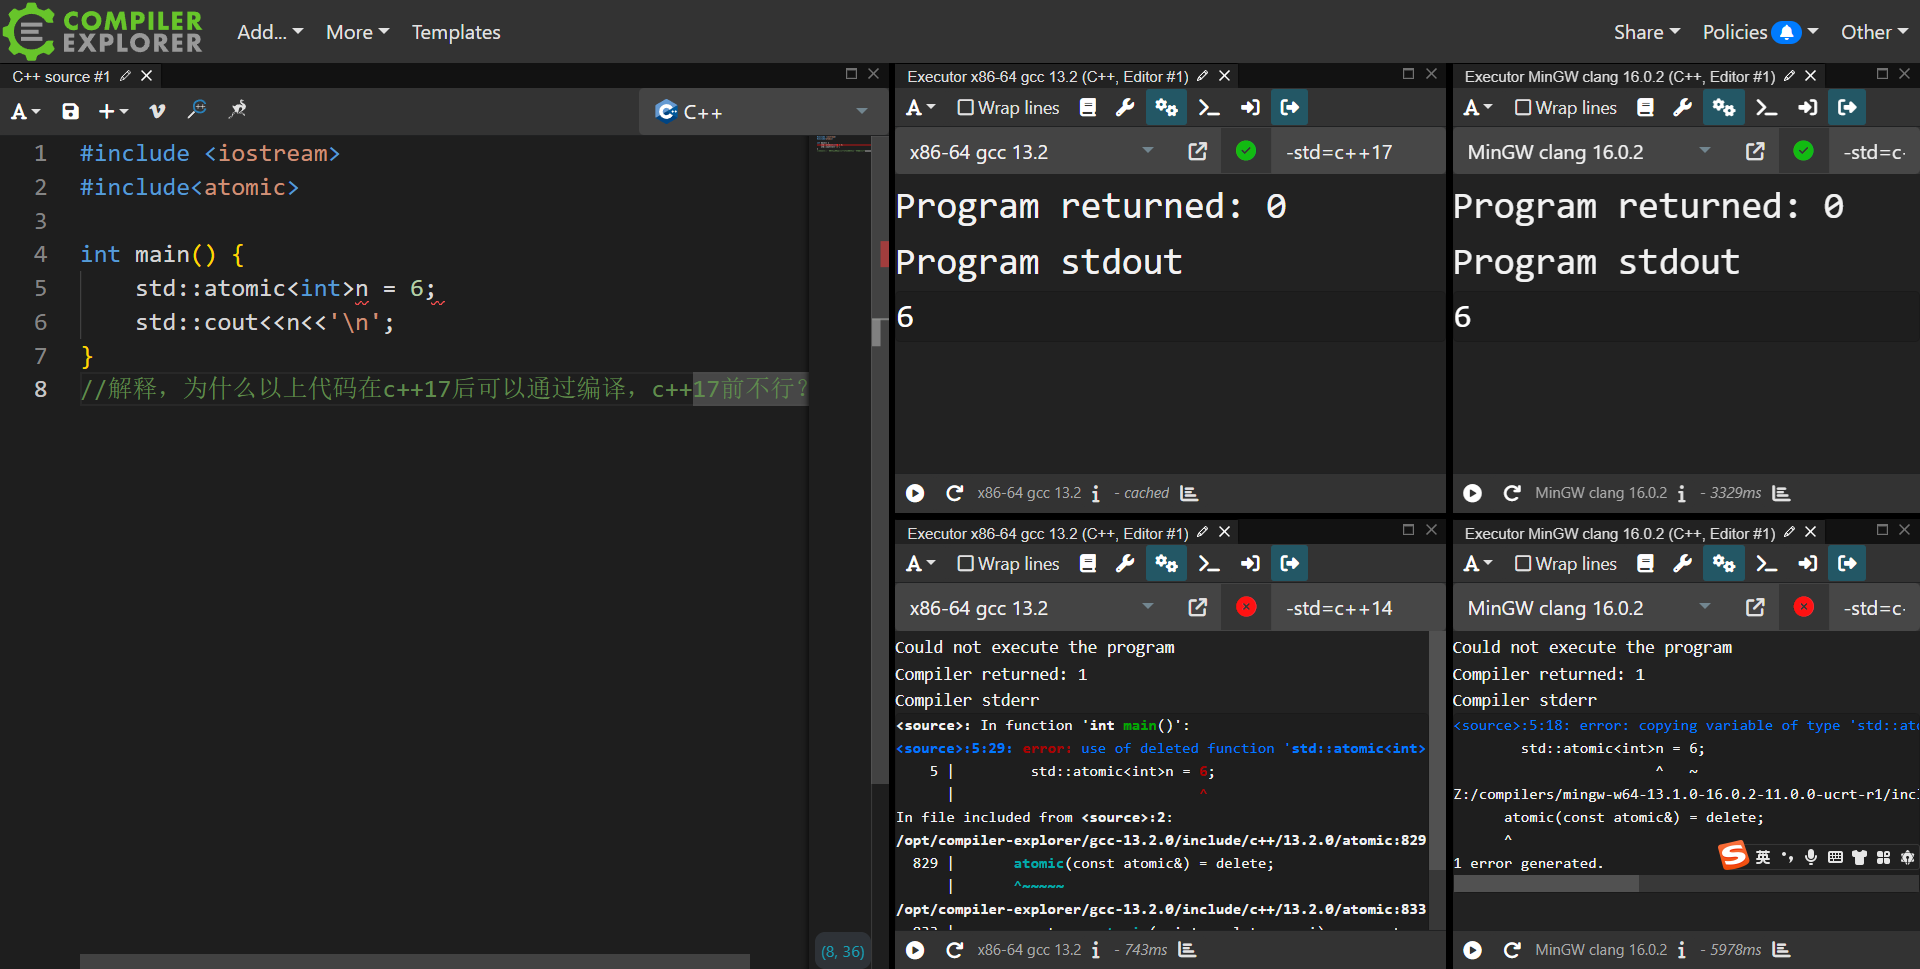
\includegraphics[width = 1.0\textwidth]{image/06_atomic.png}
\end{figure}

\begin{itemize}
    \item \textbf{难度}: \hardscore{3} \\
    \textbf{提示}:复制消除。
\end{itemize}

\section{throw new MyException}
日期:2023/8/6 出题人:mq白\\

给出代码:

\begin{minted}[mathescape,	
    linenos,
    numbersep=5pt,
    gobble=2,
    frame=lines,
    framesep=2mm]{c++}
    struct MyException :std::exception {
        const char* data{};
        MyException(const char* s) :data(s) { puts("MyException()"); }
        ~MyException() { puts("~MyException()"); }
        const char* what()const noexcept { return data; }
       };
       void f2() {
        throw new MyException("new Exception异常....");
       }
       int main(){
           f2();
       }
\end{minted}

灵感来源自 Java 人写 C++。

在 main 函数中自行修改代码,接取 f2() 函数抛出的异常(try catch)。

\begin{tcolorbox}[title = {要求运行结果},
    fonttitle = \bfseries, fontupper = \sffamily, fontlower = \itshape]
    MyException()\\
    new Exception异常....\\
    ~MyException()
\end{tcolorbox}

\begin{itemize}
    \item \textbf{难度}: \hardscore{1} \\
    \textbf{提示}:std::exception,try catch
\end{itemize}

\section{定义 array 推导指引}
日期:2023/8/12 出题人:mq白\\

给出代码:

\begin{minted}[mathescape,	
    linenos,
    numbersep=5pt,
    gobble=2,
    frame=lines,
    framesep=2mm]{c++}
    template<class Ty,size_t size>
    struct array {
        Ty* begin() { return arr; };
        Ty* end() { return arr + size; };
        Ty arr[size];
    };
    int main() {
        ::array arr{1, 2, 3, 4, 5};
        for (const auto& i : arr) {
            std::cout << i << ' ';
        }
    }
\end{minted}

要求自定义推导指引,不更改已给出代码,使得代码成功编译并满足运行结果。

\begin{tcolorbox}[title = {要求运行结果},
    fonttitle = \bfseries, fontupper = \sffamily, fontlower = \itshape]
    1 2 3 4 5 
\end{tcolorbox}

\begin{itemize}
    \item \textbf{难度}: \hardscore{3} \\
    \textbf{提示}:参考 std::array 实现,C++17类模板推导指引
\end{itemize}

\section{名字查找的问题}
日期:2023/8/15 出题人:mq白

\begin{minted}[mathescape,	
    linenos,
    numbersep=5pt,
    gobble=2,
    frame=lines,
    framesep=2mm]{c++}
    #include<iostream>

    template<class T>
    struct X {
        void f()const { std::cout << "X\n"; }
    };
    
    void f() { std::cout << "全局\n"; }
    
    template<class T>
    struct Y : X<T> {
        void t()const {
            this->f();
        }
        void t2()const {
            f();
        }
    };
    
    int main() {
        Y<void>y;
        y.t();
        y.t2();
    }
\end{minted}

给出以上代码,要求解释其运行结果。

\begin{tcolorbox}[title = {要求运行结果},
        fonttitle = \bfseries, fontupper = \sffamily, fontlower = \itshape]
    X\\
    全局
\end{tcolorbox}

\begin{itemize}
    \item \textbf{难度}: \hardscore{3} \\
          \textbf{提示}:名字查找。本问题堪称经典,在某著名 template 书籍也有提过(虽然它完全没有讲清楚)。 并且从浅薄的角度来说,本题也可以让你向其他人证明加 this 访问类成员,和不加,是有很多区别的。
\end{itemize}

\section{遍历任意聚合类数据成员}
日期:2023/8/18 出题人:mq白\\

题目的要求非常简单,在很多其他语言里也经常提供这种东西(一般是反射)。 但是显而易见 C++ 没有反射。

我们给出代码:

\begin{minted}[mathescape,	
    linenos,
    numbersep=5pt,
    gobble=2,
    frame=lines,
    framesep=2mm]{c++}
    int main() {
        struct X { std::string s{ " " }; }x;
        struct Y { double a{}, b{}, c{}, d{}; }y;
        std::cout << size<X>() << '\n';
        std::cout << size<Y>() << '\n';
    
        auto print = [](const auto& member) {
            std::cout << member << ' ';
        };
        for_each_member(x, print);
        for_each_member(y, print);
    }
\end{minted}

要求自行实现 for\_each\_member 以及 size 模板函数。 要求支持任意自定义类类型(聚合体)的数据成员遍历(聚合体中存储数组这种情况不需要处理)。 这需要打表,那么我们的要求是支持聚合体拥有 0 到 4 个数据成员的遍历。

\begin{tcolorbox}[title = {要求运行结果},
    fonttitle = \bfseries, fontupper = \sffamily, fontlower = \itshape]
    1           

    4           

    ~~0 0 0 0
\end{tcolorbox}

\begin{itemize}
\item \textbf{难度}: \hardscore{4} \\
      \textbf{提示}:\href{https://akrzemi1.wordpress.com/2020/10/01/reflection-for-aggregates/}{学习},boost::pfr。
\end{itemize}

\section{emplace\_back() 的问题}
日期:2023/8/20 出题人:\href{https://github.com/rsp4jack}{jacky}\\

思考:以下代码为什么在 C++20 以下的版本中无法成功编译,而在 C++20 及以后却可以?

\begin{minted}[mathescape,	
    linenos,
    numbersep=5pt,
    gobble=2,
    frame=lines,
    framesep=2mm]{c++}
    #include <vector>

    struct Pos {
        int x;
        int y;
    };
    
    int main(){
        std::vector<Pos> vec;
        vec.emplace_back(1, 5);
    }
\end{minted}

\begin{itemize}
\item \textbf{难度}: \hardscore{2} \\
      \textbf{提示}:new,聚合初始化。
\end{itemize}

\section{实现make\_vector()}
日期:2023/8/28 出题人:\href{https://github.com/rsp4jack}{jacky}\\

请实现函数 make\_vector(...),使以下代码编译通过(C++20):

\begin{minted}[mathescape,	
    linenos,
    numbersep=5pt,
    gobble=2,
    frame=lines,
    framesep=2mm]{c++}
    #include <cstdio>
    #include <vector>
    
    inline void dbg(const char* msg)
    {
        std::puts(msg);
        std::fflush(stdout);
    }
    
    struct X {
        X() noexcept
        {
            dbg("X()");
        };
    
        ~X() noexcept
        {
            dbg("~X()");
        };
    
        X(const X&)
        {
            dbg("X(const X&)");
        }
    
        X(X&&) noexcept
        {
            dbg("X(X&&)");
        }
    };
    
    void test()
    {
        static_assert(requires {
            {
                make_vector(std::vector{1, 2, 3})
            } -> std::same_as<std::vector<std::vector<int>>>;
            {
                make_vector(1, 2, 3)
            } -> std::same_as<std::vector<int>>;
            make_vector(1, 2, 3).size() == 3;
        });
        X    x1;
        X    x2;
        auto vec = make_vector(x1, std::move(x2));
    }
    
    int main()
    {
        test();
        dbg("test end");
    }
\end{minted}

\begin{tcolorbox}[title = {要求运行结果},
    fonttitle = \bfseries, fontupper = \sffamily, fontlower = \itshape]
    X()             \\
    X()             \\
    X(const X\&)    \\
    X(X\&\&)        \\
    X(const X\&)    \\
    X(const X\&)    \\
    ~X()            \\
    ~X()            \\
    ~X()            \\
    ~X()            \\
    ~X()            \\
    ~X()            \\
    test end
\end{tcolorbox}

\begin{itemize}
    \item \textbf{难度}: \hardscore{3} \\
          \textbf{提示}:重载决议
\end{itemize}

\section{关于 return std::move(expr)}
日期:2023/9/6 出题人:mq白\\

我们会给出三段使用到了 \mintinline{c++}{return std::move(expr)} 代码。

解释说明这些代码是否有问题,问题在哪,或者没问题,那么为什么要这样使用。

\begin{itemize}
    \item [1.]
          全局函数,返回局部对象,使用 std::move。
          \begin{minted}[mathescape,	
        linenos,
        numbersep=5pt,
        gobble=2,
        frame=lines,
        framesep=2mm]{c++}
        #include<iostream>

        struct X{//后续代码不再重复X类
            X() { puts("X()"); }
            X(const X&) { puts("X(const X&)"); }
            X(X&&)noexcept { puts("X(X&&)"); }
            ~X() { puts("~X()"); }
        };
        
        X f(){
            X x;
            return std::move(x);
        }
        
        int main(){
            X x = f();
        }
    \end{minted}
    \item [2.]
          全局函数,返回局部的引用,使用 std::move。
          \begin{minted}[mathescape,	
        linenos,
        numbersep=5pt,
        gobble=2,
        frame=lines,
        framesep=2mm]{c++}
        X&& f(){
            X x;
            return std::move(x);
        }
    \end{minted}
    \item [3.]
          类中成员函数,返回数据成员,使用 std::move。
          \begin{minted}[mathescape,	
        linenos,
        numbersep=5pt,
        gobble=2,
        frame=lines,
        framesep=2mm]{c++}
        struct Test {
            X x;
            X f() {
                return std::move(x);
            }
        };
    \end{minted}
\end{itemize}

\begin{itemize}
    \item \textbf{难度}: \hardscore{3} \\
          \textbf{提示}:return 重载决议。
\end{itemize}

\end{document}